\documentclass[border=0cm]{standalone}
\usepackage{color}
\usepackage{tikz}
\usetikzlibrary{shapes,arrows,arrows.meta,fit,positioning}

\newcommand{\defaultwidth}{5cm}
\tikzset{
    auto, node distance = 2cm,
    stage/.style = { draw, thick, rectangle, align=center,
        text width = \defaultwidth, 
        font=\bfseries,
        rounded corners=1mm, 
        minimum width = \defaultwidth
    },
    note/.style = { draw, very thin, rectangle, dashed, align=center,
        node distance = 0.5cm,
        text width = \defaultwidth - 1cm, 
        font=\footnotesize,
        minimum width = \defaultwidth - 1cm
    },
    arrow/.style = { ->, very thick }
}

\begin{document}
    \begin{tikzpicture}
        \node[stage] (0) at (0,0)
            {Set of points \\ 
\includegraphics[width=\defaultwidth]{pflock}};
        \node[stage] (1) [right = of 0]
            {Partitioning points \\ 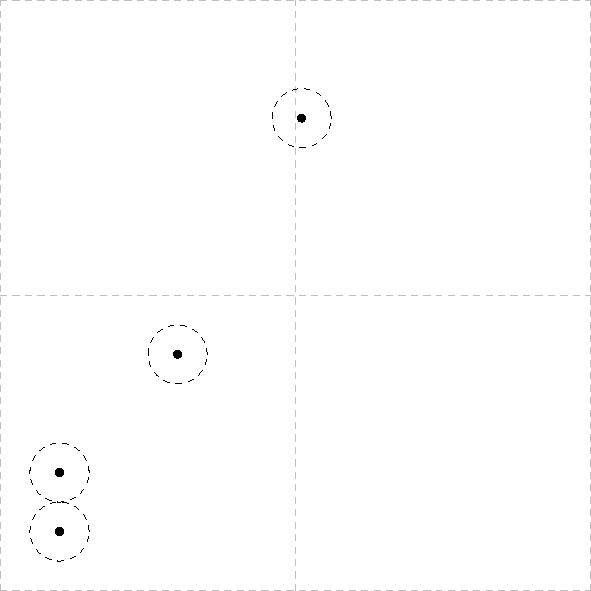
\includegraphics[width=\defaultwidth]{template}};
        \node[stage] (2) [right = of 1]
            {Finding pairs \\ 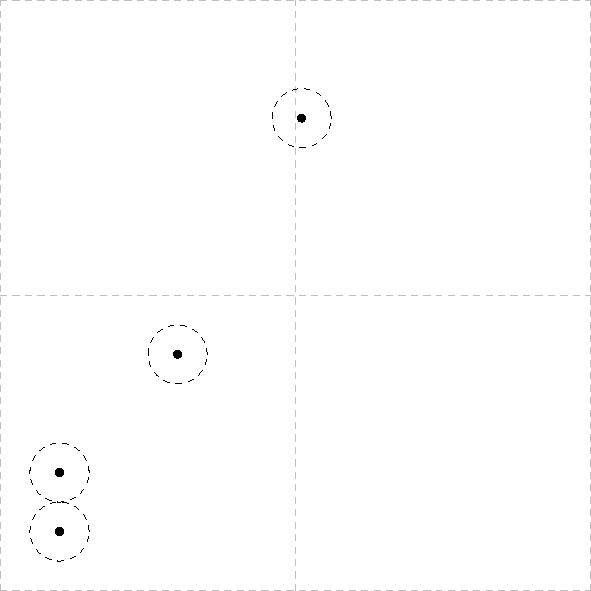
\includegraphics[width=\defaultwidth]{template}};
        \node[stage] (3) [right = of 2] 
            {Compute centers \\ 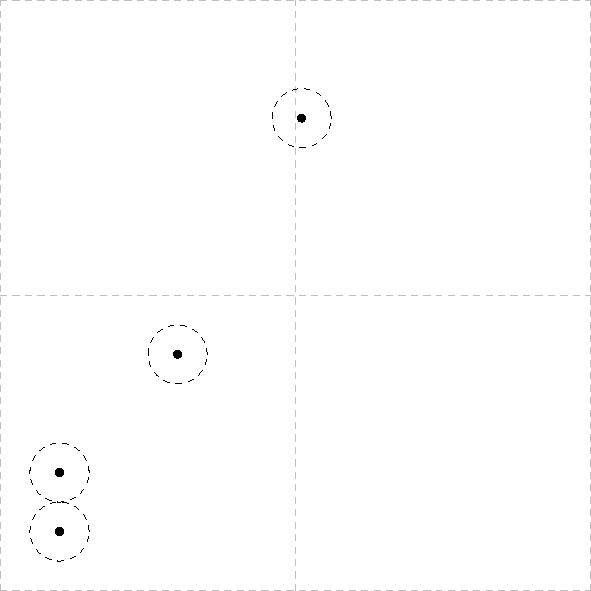
\includegraphics[width=\defaultwidth]{template}};
        \node[stage] (4) [right = of 3] 
            {Finding disks \\ 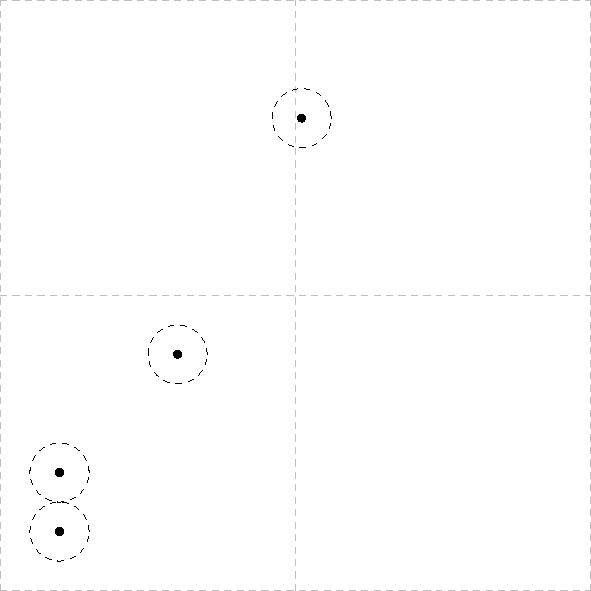
\includegraphics[width=\defaultwidth]{template}};
        \node[stage] (5) [right = of 4] 
            {Partitioning disks \\ 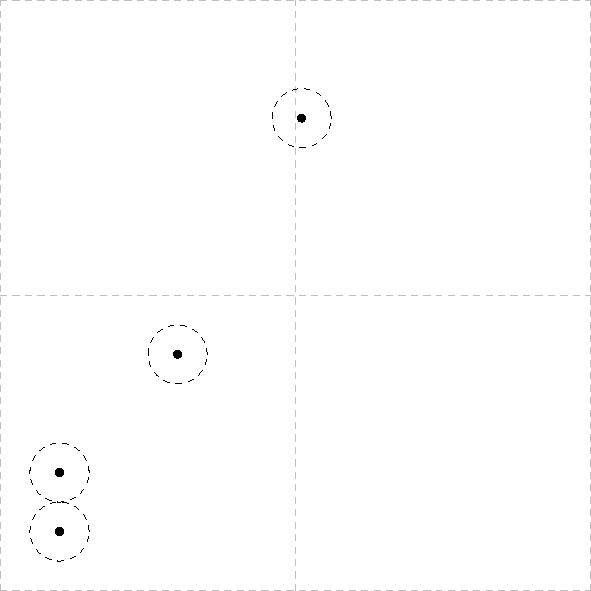
\includegraphics[width=\defaultwidth]{template}};
        \node[stage] (6) [right = of 5] 
            {LCM prunning \\ 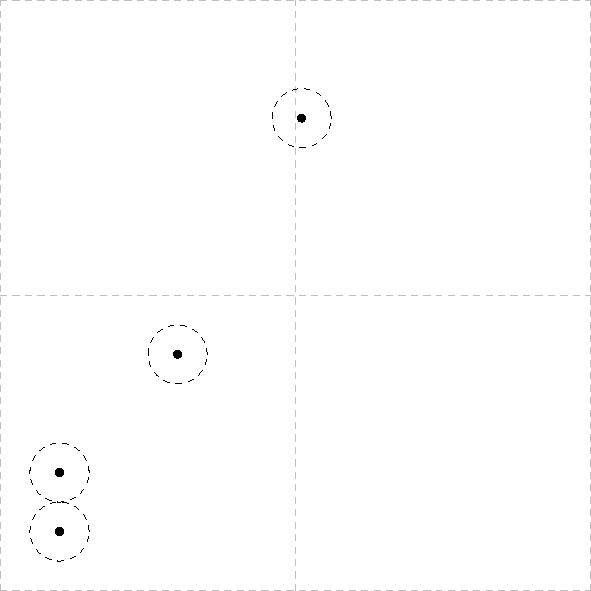
\includegraphics[width=\defaultwidth]{template}};

        \node[note] (11) [below = of 1] {Coarse grid used};            
        \node[note] (51) [below = of 5] {Fine grid used};            
                        
        \foreach \i in {1,...,6}{
            \pgfmathsetmacro\next{\i - 1}
            \path[arrow] (\next) edge (\i);
        }
    \end{tikzpicture}
\end{document}
